\section{Methods and Theory}
\label{sec:theory}

\setlength{\fboxrule}{0.1pt} 
\setlength{\fboxsep}{0.1pt}

\subsection{Extending Conformal Risk Control to Non-Monotonic Losses}
\label{subsec:finite_sample_guarantees_crc_non_monotone}

We begin with intuition. Standard CRC's proof \citep{angelopoulos2022conformal} has two key steps: First, prove that the oracle solution (using knowledge of the test point's loss), $\lambda^*$, achieves risk control; and second, show that the empirical CRC solution (with a conservative adjustment for the unknown test loss), $\hat{\lambda}$, is deterministically greater than or equal to the oracle, $\hat{\lambda}\geq \lambda^*$. Note that here, larger $\lambda$ are safer. In particular, for standard CRC, monotonicity of the loss function is then necessary and sufficient\footnote{Sufficient given the other CRC assumptions: boundedness and right-continuity of the loss, and existence of a safe $\lambda_{\max}$.} for concluding that the empirical CRC algorithm's risk is controlled: $\mathbb{E}[L_{n+1}(\hat{\lambda})] \leq \mathbb{E}[L_{n+1}(\lambda^*)]\leq \alpha$. 


Without monotonicity, what can be done? The crux is how to find a modified oracle solution, $\lambda^*_+$, and a modified empirical algorithm, $\hat\lambda_+$, such that establishing the relation $\hat\lambda_+\geq \lambda^*_+$ enables analyzing the risk of the empirical algorithm \textit{by construction}, rather than by monotonicity. Consider the family of hyperparameters defined as
\begin{align}\label{eq:methods_lambda_hat_family_def}
    &\widehat{\lambda}_+(\lbag L_{1:m}\rbag, \alpha) \\
    & \ := \inf \Big\{\lambda_0 \in \Lambda \ : \ \forall \ \lambda\geq \lambda_0,
    \ \ \sum_{i=1}^{m}\frac{L_i(\lambda)}{m} \leq \alpha \Big\}, \nonumber
\end{align}
when the set is nonempty, and otherwise define $\widehat{\lambda}_+(\lbag L_{1:m}\rbag, \alpha):=\lambda_{\max}$, where $\lambda_{\max}$ is a ``safe hyperparameter'' assumed to exist as in \citet{angelopoulos2022conformal}:  $\lambda_{\max}:=\sup\Lambda\in \Lambda$ and $L_i(\lambda_{\max})\leq \alpha$.
In words, $\widehat{\lambda}_+$ is the smallest (most aggressive) hyperparameter such that the empirical risk is controlled at level $\alpha$ \textit{for all hyperparameters at least as large as it}; this ``for all $\lambda\geq \lambda_0$'' qualification is the key algorithmic modification to standard CRC. 
We then define the oracle solution by Eq. \eqref{eq:methods_lambda_hat_family_def} fit on the bag (or multiset) containing both the calibration and test loss functions, $\lbag L_{1:n+1}\rbag$:
\begin{align}\label{eq:methods_lambda_oracle_def}
    \lambda_+^*:= \widehat{\lambda}_+(\lbag L_{1:n+1}\rbag, \alpha).
\end{align}
Similarly, define the empirical algorithm as Eq. \eqref{eq:methods_lambda_hat_family_def} fit on the bag of the calibration losses, with the bound $B$ in place of $L_{n+1}$ to conservatively adjust for the unknown test loss:
\begin{align}\label{eq:methods_lambda_empirical_def}
    \hat{\lambda}_+:= \widehat{\lambda}_+(\lbag L_{1:n}, B\rbag, \alpha).
\end{align}
Our empirical algorithm, $\hat{\lambda}_+$, reduces to CRC when the losses are monotonic, and it can be viewed as searching hyperparameter space from \textit{a priori} safest to most aggressive, the opposite direction of standard CRC (Figure \ref{fig:CRC_counterexample}). Also note that our generalized CRC (gCRC) is conservatively designed to be \textit{a priori} safer than the oracle, that is, $\hat\lambda_+\geq \lambda^*_+$ almost surely. Unfortunately, this construction is not itself sufficient for $\hat{\lambda}_+$ to achieve validity at level $\alpha$ (Appendix \ref{app:counterexample}). Relating the empirical algorithm to the oracle, however, does provide finite-sample guarantees for $\hat\lambda_+$ under Lipschitz continuity and depending on algorithmic stability. 



\begin{definition}[$\epsilon$-replace-one stability]
    \label{eq:def_replace_one_stability}
    We say that a function  $h$ is $\epsilon$-replace-one stable if for all $i, j\in [n+1]$, 
    % $i\neq j$, 
    \begin{align*}
        \mathbb{E}\Big[\big|h(\lbag Z_{1:n+1}\rbag\backslash \{z_i\})-h(\lbag Z_{1:n+1}\rbag\backslash \{Z_j\})\big|\Big] \leq \epsilon.
    \end{align*}
\end{definition}
% \textbf{Definition: $\epsilon$-replace-one stability.} We say that a function  $h$ is $\epsilon$-replace-one stable if for all $i, j\in [n+1], i\neq j$, 
% \begin{align*}
%     \mathbb{E}\Big[\big|h(\lbag L_{1:n+1\backslash i})-h(\lbag L_{1:n+1\backslash j})\big|\Big] \leq \epsilon.
% \end{align*}
The following result then provides finite-sample guarantees for $\hat\lambda_+$ even for non-monotonic losses.
\begin{theorem}
\label{thm:gcrc_nonmonotonic}
    Assume exchangeable $L_i(\lambda)$. Define  $\lambda_{\max}:=\sup\Lambda\in \Lambda$ and assume 
    \begin{align*}
        L_i(\lambda_{\max})\leq \alpha, \qquad \sup_{\lambda}L_i(\lambda)\leq B < \infty \quad \text{almost surely}.
    \end{align*}
    If the $L_i(\lambda)$ are $K$-Lipschitz in $\lambda$ and $\hat\lambda_+$ is $\epsilon$-replace-one stable, then
    % Then, if the Lipschitz constant $K$ is known and $\hat\alpha$ exists, 
    % \begin{align*}
    %     \mathbb{E}\big[L_{n+1}\big(\hat{\lambda}_{+}(\hat\alpha)\big)\big] \leq \alpha,
    % \end{align*}
    % and if $K$ is not known but $\hat\lambda_+$ is $\epsilon$-replace-one stable, then
    \begin{align*}
        \mathbb{E}\big[L_{n+1}(\hat\lambda_+)\big] \leq \alpha + K\epsilon.
    \end{align*}
\end{theorem}
\textbf{Proof sketch:} Conditional on the bag of data, $\lbag z_{1:n+1} \rbag$, we show that the oracle $\lambda_+^*$ achieves risk control, which implies risk control for all $\lambda\geq\lambda_+^*$ that are constant conditional on $\lbag z_{1:n+1} \rbag$. We then show $\hat\lambda_+\geq \lambda_+^*$ almost surely. Lastly, using Lipschitz continuity and replace-one stability, we relate the risk of $\hat\lambda_+$ to that of some $\lambda\geq\lambda_+^*$ that is constant conditional on $\lbag z_{1:n+1} \rbag$. We defer the proof to App. \ref{app:gcrc_proof_nonmonotonic_1dim}.

\begin{remark}[Attaining $\alpha$-validity if $K$ is known]
    If $K$ is known, then a more conservative significance level, $\hat\alpha \leq \alpha$, can be used for level $\alpha$ validity, regardless of instability:
    \begin{align*}
        \mathbb{E}\big[L_{n+1}\big(\hat{\lambda}_{+}(\hat\alpha)\big)\big] \leq \alpha,
    \end{align*}
    where $\hat\alpha$ is defined in Appendix \ref{app:conservative_adjustment_K_known}.
\end{remark}

\begin{remark}[Monotone envelope interpretation]
    The $\hat{\lambda}_+$ in Eq. \eqref{eq:methods_lambda_empirical_def} can be viewed as the smallest hyperparameter such that the ``monotonized empirical risk'' is controlled at $\alpha$. The procedure is presented with this interpretation in \citet{angelopoulos2022conformal}'s App. A, but that paper noted that finite-sample guarantees for $\hat{\lambda}_+$ were at the time unknown. 
\end{remark}

\begin{algorithm}[!t]
    \caption{Pseudo-code for $\beta$ calibration.}
    \label{alg:calibrate_beta}
    \begin{algorithmic}
        \REQUIRE Safe policy $\pi_0$; optimized policies $\pi_1, ..., \pi_t$; sets of prompts $X^{(0)}, ..., X^{(t)}$; calibration data $\mathcal{D}_{\text{cal}}$; proposal data $\mathcal{D}_{\text{prop}} \sim \pi_t$; target risk $\alpha$; loss upper bound $B$.
        \ENSURE Likelihood ratio bound $\hat{\beta}$
        \STATE $\rho_i \gets \pi_t(A_i | X^{(t)}) \,/\, \pi_0(A_i | X^{(0)})$ for $i \in \mathcal{D}_{\text{cal}} \cup \mathcal{D}_{\text{prop}}$
        \STATE $G \gets \textsc{PrepareGrid}(\{\rho_i\})$
        \STATE Initialize: $\hat{\beta} \gets \beta_{\min}$
        \FOR{$\beta \in G$ (ascending)}
            \STATE \# \text{Compute constrained PDF, mixture of past PDFs}
            \STATE $\psi_\beta \gets \textsc{EstimatePsi}(\{\rho_i\}, \beta)$ 
            % \STATE $w_i \gets \min(\rho_i, \beta) \,/\, \psi_\beta$ for $i \in \mathcal{D}_{\text{cal}}$
            % \STATE $\pi_t^{(\beta)}(A_i) \gets \min(\rho_i, \beta) \,/\, \psi_\beta$ for $i \in \mathcal{D}_{\text{cal}}$
            \STATE $\pi_t^{(\beta)}(A_i) \gets \min(\pi_t(A_i), \beta\cdot \pi_0(A_i)) \,/\, \psi_\beta$ for $i \in \mathcal{D}_{\text{cal}}$
            \STATE $\pi_{0:t-1}^{\text{mix}}(A_i) \gets \textsc{MixPDF}(A_i, \pi_{0:t-1})$ for $i \in \mathcal{D}_{\text{cal}}$
            \STATE
            \STATE \# \text{Compute conformal weights, check empirical risk}
            \STATE $w_i \gets \pi_t^{(\beta)}(A_i) / \pi_{0:t-1}^{\text{mix}}(A_i)$ for $i \in \mathcal{D}_{\text{cal}}$
            \STATE $w_{\max} \gets \textsc{EstimateWMax}(\{w_i\}, \pi_0, \pi_t)$
            \STATE $\tilde{w}_i \gets w_i/(\sum_{j \in \mathcal{D}_{\text{cal}}} w_j + w_{\max})$ for $i\in \mathcal{D}_{\text{cal}}$
            \IF{$\sum_{i \in \mathcal{D}_{\text{cal}}} \tilde{w}_i \cdot l_i + \tilde{w}_{\max} \cdot B > \alpha$}
                \STATE \textbf{Return:} $\hat{\beta}$
            \ENDIF
            \STATE $\hat{\beta} \gets \beta$
        \ENDFOR
        \STATE \textbf{Return:} $+\infty$
    \end{algorithmic}
\end{algorithm}


\subsection{Conformal Policy Control: Selecting a Risk-Controlling Policy}
\label{subsec:cpc_selecting_rc_policy}


We first state the only critical assumptions required by CPC: access to a safe policy and subsequent optimized policies. For ease of notation we will describe CPC in an online setting where one action is taken or sample generated each policy improvement step, but it also works similarly in a multiround batch setting.


\textbf{Assumption 1: An Initial Safe Policy} Assume access to an initial safe policy, $\pi_{0}$, for which the true risk is controlled at the desired level $\alpha$; that is, assume $\mathbb{E}_{X \sim p} \ \mathbb{E}_{A \sim \pi_{0}(\cdot \mid X)} \ [\ell(X, A)] \leq \alpha$
holds for $\pi_{0}$.
Note that this assumption is weaker than it may appear: any existing policy (a previous deployment, a domain default, or even a uniform baseline) qualifies as $\pi_0$ so long as its risk is at most $\alpha$. When little is known, $\alpha$ can be set loosely and any reasonable baseline suffices; the strength of the resulting guarantee scales with how much is actually known about what is safe.

\textbf{Assumption 2: Access to Each Optimized Policy} At each time $t = 1, 2, ...$, also assume access to the optimized model, $\pi_{t}$, which may be trained to maximize expected reward (as in the ``unconstrained'' part of Eq. \eqref{eq:constrained_policy_opt}). We do not require any assumptions on how $\pi_{t}$ is trained, although better optimized performance (with respect to both the constraint and the reward) may translate into better efficiency and reward of the constrained policy.


\textbf{Constraining Policies by Clipping Likelihood Ratios} We define the constrained policy $\pi_{t}^{(\beta)}$ by clipping the likelihood ratio $\pi_t / \pi_0$ at a bound $\beta > 0$ and renormalizing. Actions whose likelihood ratio exceeds $\beta$ are capped at $\beta \cdot \pi_0$, limiting how far the constrained policy can deviate from the safe policy. That is,
\begin{align}\label{eq:piecewise_constraint_def}
\pi_{t}^{(\beta)}(a \mid x) \propto \min\big(\pi_{t}(a \mid x), \ \beta\cdot \pi_{0}(a \mid x)\big) .
\end{align}
Assume there is some small, positive $\beta_{\min}\ll1$ such that $\beta_{\min}\leq \pi_t(a \mid x)/\pi_0(a \mid x)$ for all $x\in \mathcal{X}$, $a \in \mathcal{A}$. As $\beta \to \beta_{\min}$ the constrained policy approaches the safe one, $\pi_t^{(\beta)} \to \pi_0$, and as $\beta \to \infty$ it approaches the optimized one, $\pi_t^{(\beta)} \to \pi_t$ (Figure \ref{fig:interpolating_distributions}). Crucially, because $\beta$ governs the likelihood ratio and not the loss, any smoothness needed for a guarantee will be smoothness the agent can compute and verify. Theorem \ref{thm:cpc} makes this precise.



\textbf{Calibrating $\boldsymbol{\beta}$:} We calibrate $\beta$ analogously to $\hat\lambda_+$ (Section \ref{subsec:finite_sample_guarantees_crc_non_monotone}), searching from what we \textit{a priori} expect is safest to most aggressive. For $\beta$, this means searching in increasing order in a grid (or set of intervals) $G\subset (0, \infty]$, to find the largest value where the conservatively-adjusted weighted empirical risk is still controlled (Algorithm \ref{alg:calibrate_beta}):
\begin{align}\label{eq:beta_hat_def_methods}
    &\hat{\beta}\big(\lbag L_{0:t-1}, B \rbag, (\tilde{w}_{0:t-1}^{(\cdot)}, \tilde{w}_{\max}^{(\cdot)}),  \alpha\big) \\
    & := \sup \Big\{\beta' \in G \ : \ \forall \ \beta \leq \beta', \ B\tilde{w}_{\max}^{(\beta)} + \sum_{i=0}^{t-1}l_i\tilde{w}_i^{(\beta)} \leq \alpha \Big\}, \nonumber
\end{align}
where the $\tilde{w}_i^{(\beta)}$ and $\tilde{w}_{\max}^{(\beta)}$ are (normalized) conformal importance weights. These weights correct for the distribution shift between the policies that generated the calibration data and the candidate policy $\pi_t^{(\beta)}$: since the agent's past actions were drawn from earlier policies, each observation must be reweighted to obtain a valid risk estimate under $\pi_t^{(\beta)}$. This is the importance weighting described in Section~\ref{sec:background}, now made precise for the multi-round setting.

Formally, we define $\tilde{w}_i^{(\beta)}$ as in \citet{prinster2024conformal} via the likelihoods of all permutations of the calibration data $z_{0:t-1}$ and a hypothetical test sample $z_t \in \mathcal{Z} := \mathcal{X} \times \mathcal{A}$. A key subtlety is that $z_t$ is not yet known, as CPC calibration occurs prior to sampling. For any $z_t$, define the unnormalized weight
\begin{align*}
    w_i^{(\beta)}:=\sum_{\sigma:\sigma(t)=i}\pi_{0:t}^{(\beta)}(z_{\sigma(0)}, ..., z_{\sigma(t)})
\end{align*}
for all $i\in\{0, ..., t\}$ and for permutations $\sigma$ of the indices. For $i\in\{0, ..., t\}$, further denote the normalized weights as
\begin{align*}
    \tilde{w}_i^{(\beta)}:= w_i^{(\beta)}/\sum_{i=0}^tw_i^{(\beta)}, \hspace{4mm}\tilde{w}_{\max}^{(\beta)}:=\sup_{z_t\in \mathcal{Z}}(\tilde{w}_t^{(\beta)}),
\end{align*}
where $\tilde{w}_{\max}^{(\beta)}$ is a conservative estimate of the test point weight.
% \begin{align*}
%     \tilde{w}_{\max}^{(\beta)}:=\sup_{z_t\in \mathcal{Z}}(\tilde{w}_t^{(\beta)}).
% \end{align*}
Hereon, we refer to normalized calibration and (conservative) test point weights, that is, assuming $\sum_{i=0}^{t-1}\tilde{w}_{i}^{(\beta)}+\tilde{w}_{\max}^{(\beta)}=1$.
In practice these weights are not computationally tractable, but we estimate the $\tilde{w}_i^{(\beta)}$ by approximating past policies as one mixture distribution, $\pi_{0:t-1}^{\text{mix}}\approx \pi_{0:t-1}$, which yields a fast linear runtime; additionally, we estimate $\tilde{w}_{\max}^{(\beta)}$ by an empirical maximum over samples from $\pi_0$ and $\pi_t$. If the weights are computed exactly, CPC achieves the following guarantee.
% ---note that $\hat\alpha$ for this result is defined in Appendix \ref{app:cpc_proof}, where we also provide the proof.

% \begin{theorem}
% \label{thm:cpc}
%     Assume that $L_i\cdot w_i^{(\beta)}$ is $K$-Lipschitz in $\beta$, that $\mathbb{E}_{\pi_0}[L_t]\leq \alpha$, and  $L_i\leq B < \infty$ for all $i$.
%     Then, if the Lipschitz constant $K$ is known and $\hat\alpha$ exists, 
%     \begin{align*}
%         \mathbb{E}_{\pi_{0:t}^{(\hat\beta(\hat\alpha))}}\big[L_{t} \big] & \leq \alpha.
% \end{align*}
%     and if $K$ is not known but $\hat\beta$ is $\epsilon$-replace-one stable, then
%     \begin{align*}
%         \mathbb{E}_{\pi_{0:t}^{(\hat\beta)}}\big[L_{t} \big] & \leq \alpha + K\cdot \epsilon .
% \end{align*}
% \end{theorem}
\begin{theorem}
\label{thm:cpc}
    Assume that $\mathbb{E}_{\pi_0}[L_t]\leq \alpha$,  $L_i\in[0,B], B<\infty$ for all $i$, and $\hat\beta$ is $\epsilon$-replace-one stable. If $w_i^{(\beta)}$ is $K$-Lipschitz in $\beta$ for all $i$, then
    \begin{align*}
        \mathbb{E}_{\pi_{0:t}^{(\hat\beta)}}\big[L_{t} \big] \leq \alpha + BK\epsilon.
    \end{align*}
    If $(l_i - \alpha) \cdot w_i^{(\beta)}$ is $K'$-Lipschitz in $\beta$, then
    \begin{align*}
        \mathbb{E}_{\pi_{0:t}^{(\hat\beta)}}\big[L_{t} \big] \leq \alpha + K'\epsilon.
    \end{align*}
\end{theorem}

\begin{figure}[!t]
\centering
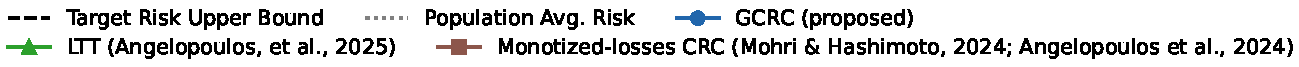
\includegraphics[width=\linewidth]{figures/legend_logprobs_risk.pdf}\\[0.5em]
\begin{subfigure}{0.48\linewidth}
    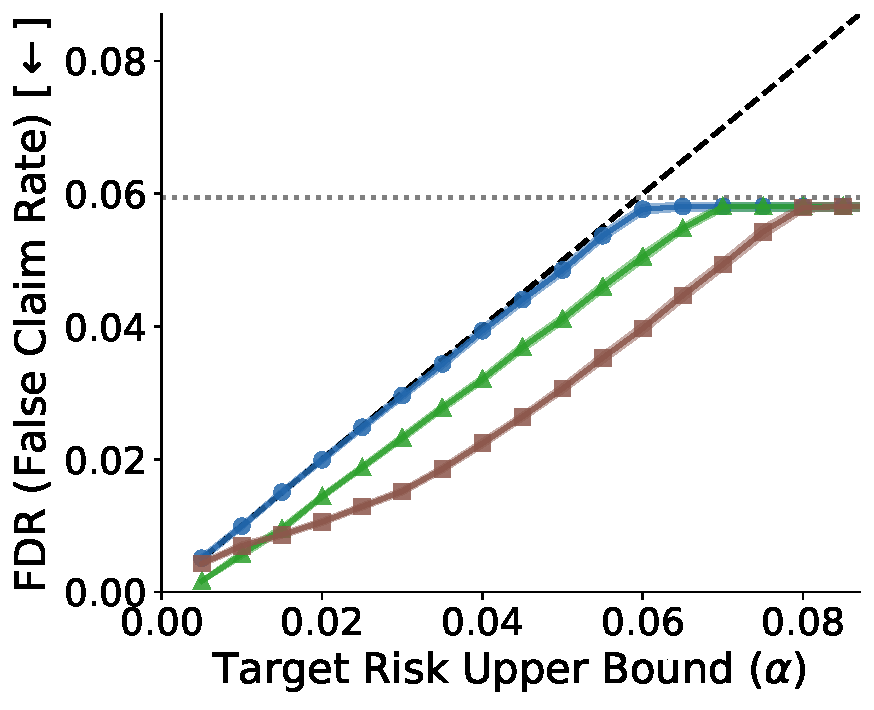
\includegraphics[width=\linewidth]{figures/loss_factuality_fdrLoss_logprobsScoring_risk_25trials_200ngrid.pdf}
\end{subfigure}
\hfill
\begin{subfigure}{0.48\linewidth}
    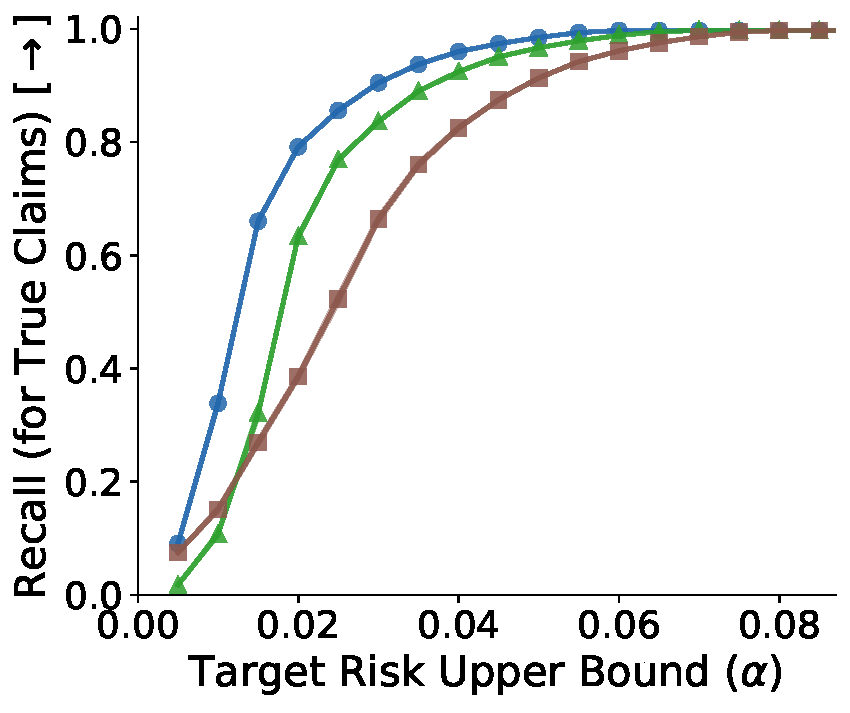
\includegraphics[width=\linewidth]{figures/loss_factuality_fdrLoss_logprobsScoring_claims_25trials_200ngrid.pdf}
\end{subfigure}
\caption{Medical QA factuality control results on MedLFQA. \textbf{Left:} Empirical FDR (fraction of retained claims that are false) vs.\ target risk level $\alpha$. The dashed line indicates $y = x$; valid methods should fall at or below this line. \textbf{Right:} Recall (fraction of true claims retained) vs.\ $\alpha$. gCRC tightly controls FDR at the target level while achieving superior recall to baselines. Results averaged over 25 random splits. Error regions are standard errors.}
\label{fig:MedicalQA}
\end{figure}




A key advantage of CPC over gCRC is where the Lipschitz condition falls. In Theorem \ref{thm:gcrc_nonmonotonic}, smoothness is required of $l_i(\lambda)$, the loss as a function of the control parameter, which is a property of the unknown environment. In Theorem \ref{thm:cpc}, smoothness is required of $w_i^{(\beta)}$ or $(l_i - \alpha)\cdot w_i^{(\beta)}$ as a function of $\beta$. Since $l_i$ does not depend on $\beta$, this regularity is determined entirely by the conformal weights, which depend on the likelihood ratio between the safe and optimized policies. The assumption thus concerns the agent's own policies rather than the unknown constraint function, and is in principle verifiable or enforceable by the practitioner.


\textbf{Sampling from the Constrained Policy in Combinatorial Action Spaces}
In large action spaces, the normalization constant of $\pi_t^{(\hat\beta)}$ is intractable. However, accept-reject (AR) sampling \citep{von1963various} avoids normalization entirely. When $\hat\beta$ is small, proposals from $\pi_0$ are efficient, with the AR envelope constant set to $\hat\beta$. When $\hat\beta$ is large, proposals from $\pi_t$ are more efficient, since $\pi_t^{(\hat\beta)} \approx \pi_t$. See Figure \ref{fig:interpolating_distributions} for an illustration and Appendix \ref{app:sampling} for details.

\begin{figure*}[!t]
\centering
    \begin{subfigure}{\textwidth}
        \centering
        
\includegraphics[width=\textwidth]{figures/legend_ActiveLearningExpts.pdf}
    \end{subfigure}
    \\
    \begin{subfigure}{0.3\textwidth}
        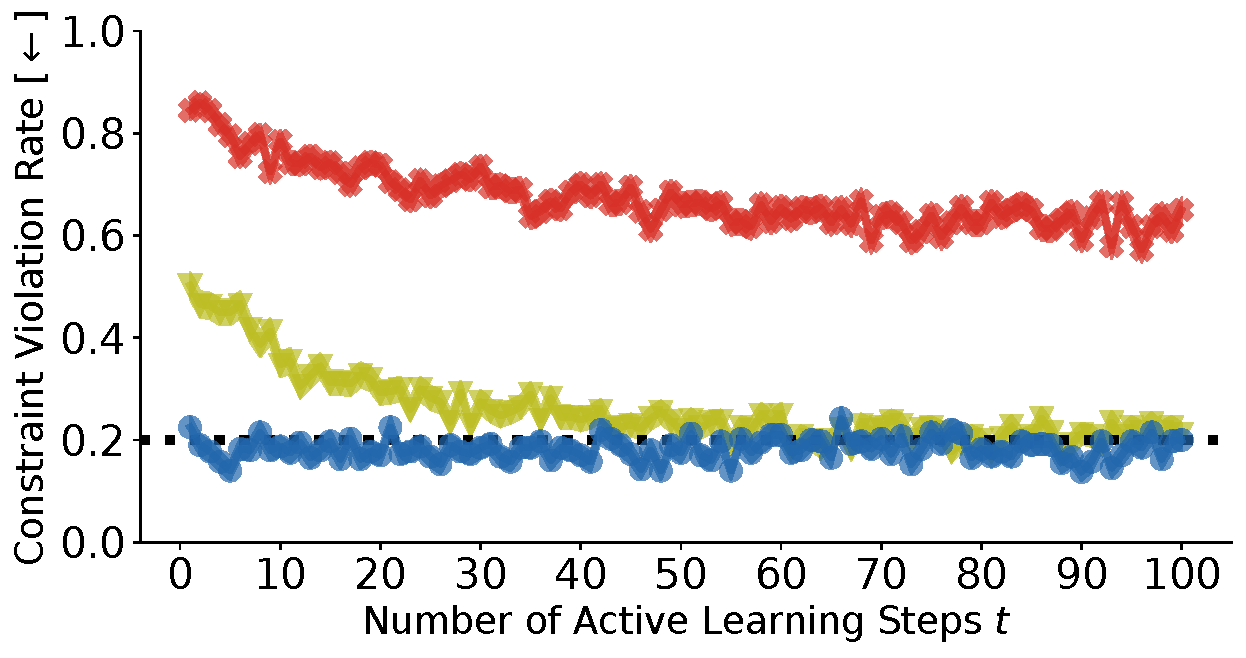
\includegraphics[width=\textwidth]{figures/SplitCPActiveLearning_robot_arm_infeasiblity_20260209.pdf}
    \end{subfigure}
    \hspace{0.1cm}
    \begin{subfigure}{0.3\textwidth}
        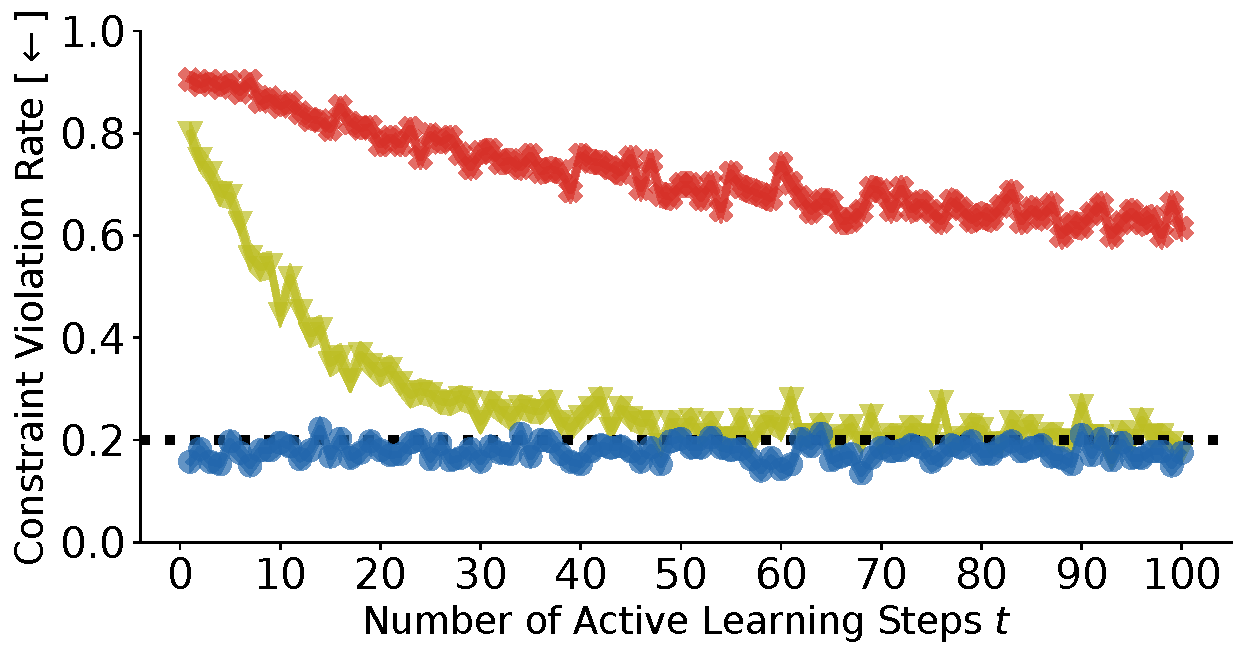
\includegraphics[width=\textwidth]{figures/SplitCPActiveLearning_airfoil_infeasiblity_20260209.pdf}
    \end{subfigure}
    \hspace{0.1cm}
    \begin{subfigure}{0.3\textwidth}
        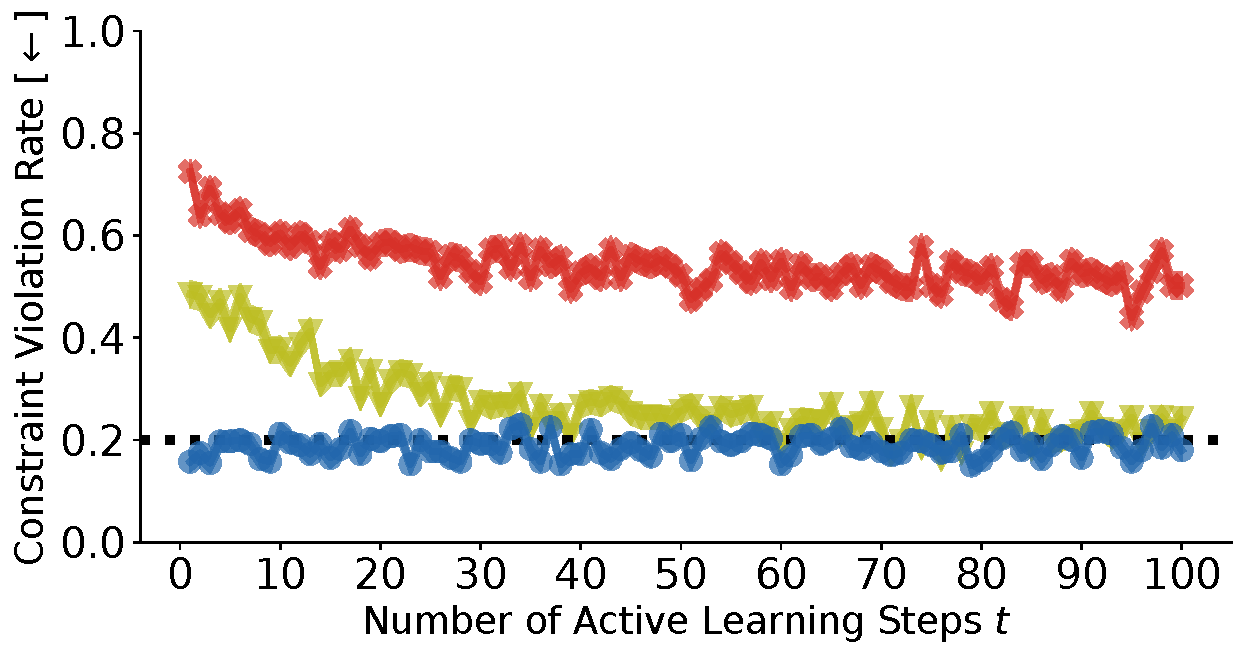
\includegraphics[width=\textwidth]{figures/SplitCPActiveLearning_meps_infeasiblity_20260209.pdf}
    \end{subfigure}
    \\
    \begin{subfigure}{0.3\textwidth}
        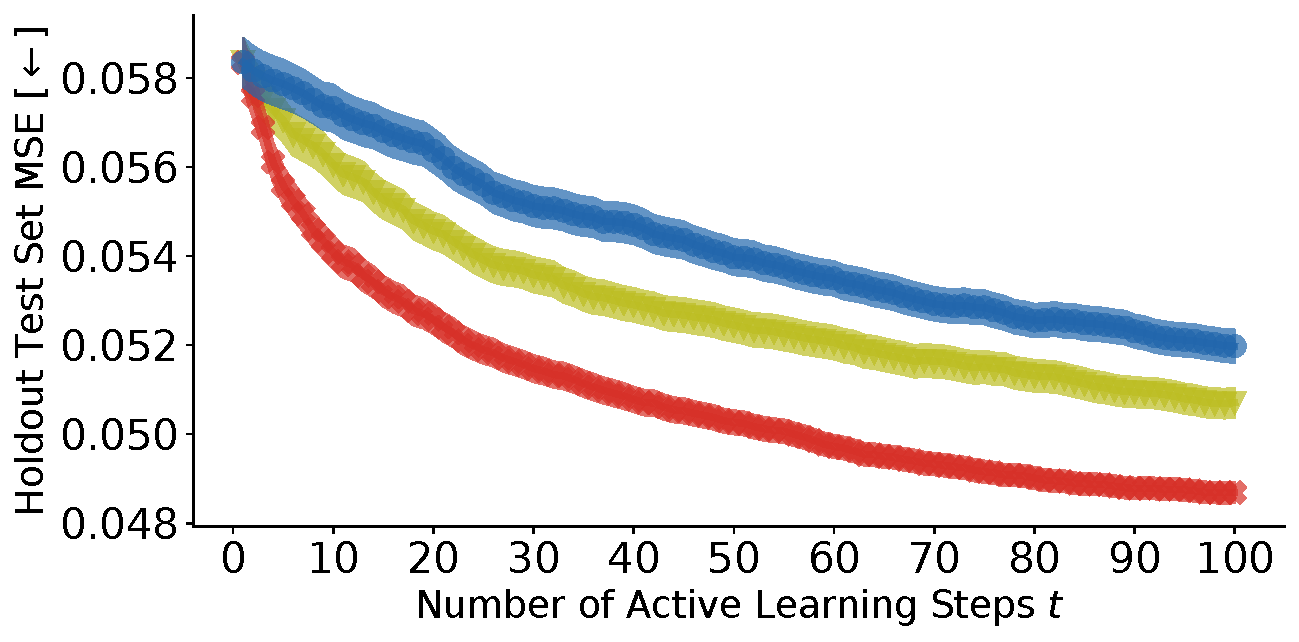
\includegraphics[width=\textwidth]{figures/SplitCPActiveLearning_robot_arm_MSE_20260209.pdf}
    \end{subfigure}
    \hspace{0.1cm}
    \begin{subfigure}{0.3\textwidth}
        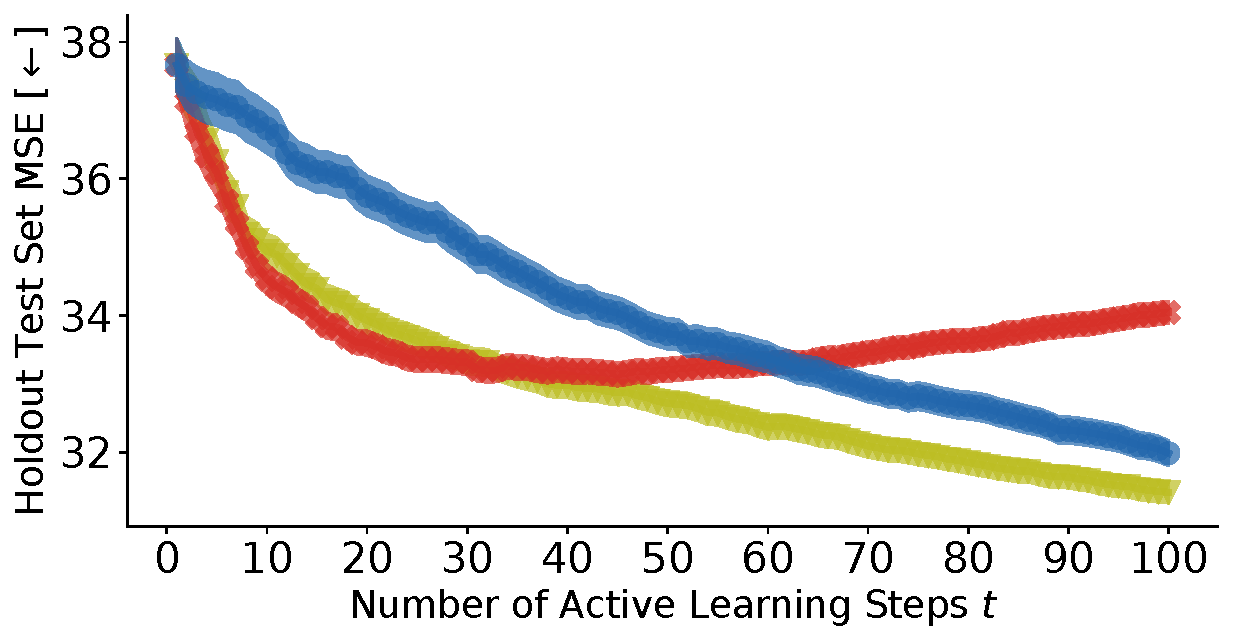
\includegraphics[width=\textwidth]{figures/SplitCPActiveLearning_airfoil_MSE_20260209.pdf}
    \end{subfigure}
    \hspace{0.1cm}
    \begin{subfigure}{0.3\textwidth}
        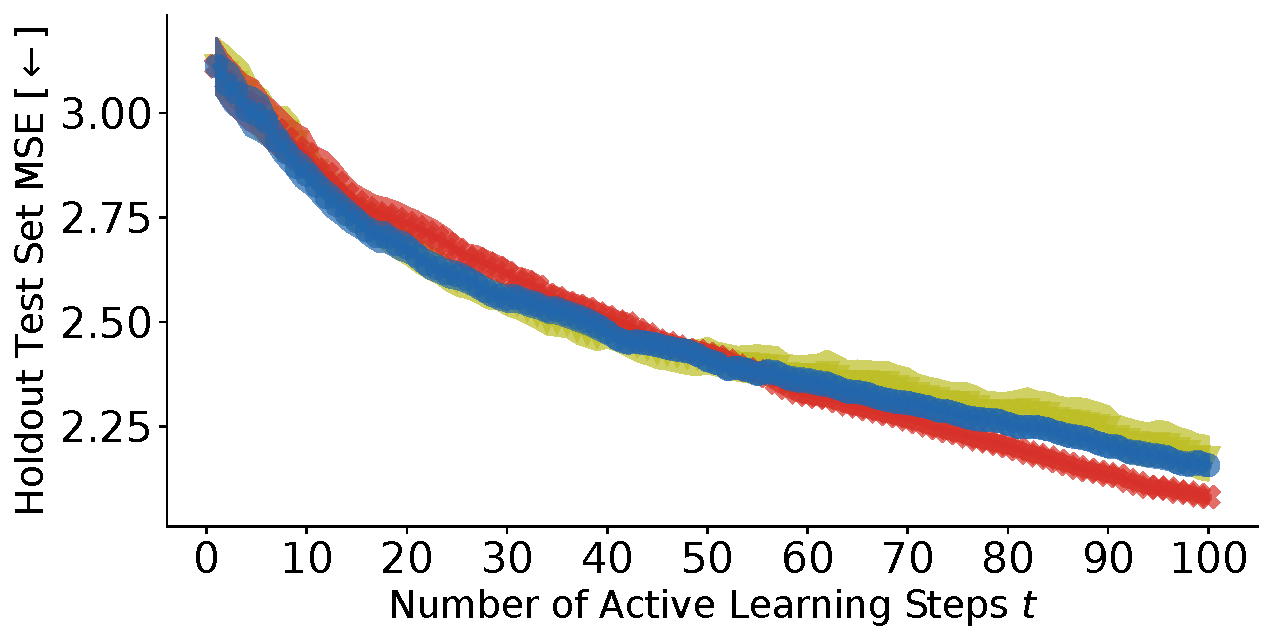
\includegraphics[width=\textwidth]{figures/SplitCPActiveLearning_meps_MSE_20260209.pdf}
    \end{subfigure}
    \\
    \begin{subfigure}{0.33\textwidth}
        \centering
        \textbf{Robot Arm Kinematics}
    \end{subfigure}
    \hfill
    \begin{subfigure}{0.33\textwidth}
        \centering
        \textbf{Airfoil}
    \end{subfigure}
    \hfill
    \begin{subfigure}{0.33\textwidth}
        \centering
        \textbf{Healthcare Utilization (MEPS)}
    \end{subfigure}
\caption{Conformal policy control in the active learning setting. We train Gaussian process regression models on tabular datasets, providing a small amount of initial data for training and selecting the remaining training data via exponential tilting toward the posterior predictive variance. We introduce a feasibility constraint based on alignment with the leading principal component of the Gram matrix to make the task more difficult. CPC controls the constraint violation risk at our desired threshold $\alpha = 0.2$, while simultaneously reducing test MSE. Surprisingly, in some cases the risk-controlled data selection policy attains lower test MSE than the uncontrolled policy.}
\label{fig:AL_enumerated_options}
\end{figure*}